% o Inhoudelijke verkenning, kennis benodigd voordat met het ontwerp gestart kan worden (o.a. normen en regelgeving), 
% vaak a.d.h.v. gerelateerd werk.
% o Relevante onderzoeksvragen worden hierin uitgewerkt.
% o Welke literatuur en/of theorieën zijn relevant en wat betekent dit voor het
% ontwerp.
% o Overzicht van bestaande oplossingen van het probleem en waarom voldoen
% deze in dit specifieke geval wel/niet

\section{Invloeden op productiviteit} \label{sec:theory}
Volgens een groot aantal onderzoeken hebben de volgende factoren de meeste invloed op productiviteit\cite{comfort-grootheden}:
\begin{itemize}
    \item Luchtkwaliteit
    \begin{itemize}
        \item VOC (Volatile Organic Compounds)
        \item Luchtvochtigheid
    \end{itemize}
    \item Geluidsniveau
    \item Lichtkwaliteit
\end{itemize}


\subsection{Luchtkwaliteit}
% Vertel over verschillende grootheden binnen luchtkwaliteit die gemeten kunnen worden met sensor.
% Vertel welke sensoren geimplementeerd kunnen worden. Dit is niet onderzoek. Het antwoord is Luchtvochtigheidssensor en PPM-Bullshit-In-De-Lucht-Sensor.
% Concludeer dat we 2 sensoren nodig hebben: luchtvocht en luchtqual
Luchtkwaliteit bestaat uit verschillende aspecten. Twee hiervan zijn VOC (Volatile Organic Compounds) en luchtvochtigheid\cite{comfort-grootheden}\cite{luchtkwal-is-voc-denk-ik-misschien}. Dit zijn de twee luchtkwaliteit gerelateerde waardes die gemeten gaan worden.

Luchtvochtigheid wordt normaal gemeten in \textit{relatieve} luchtvochtigheid. Dit geeft aan hoeveel waterdamp er in de lucht zit, vergeleken met hoeveel waterdamp er in de lucht kan zitten op de huidige temperatuur. Een relatieve luchtvochtigheid van 100\% is de maximale hoeveelheid waterdamp die er met de huidige temperatuur in de lucht kan zitten. 

\subsection{Kamertemperatuur}
De temperatuur waar een persoon zich comfortabel bij voelt hangt niet alleen af van de temperatuur zelf maar ook de luchtvochtigheid in een ruimte\cite{palonen1993effects}. Dit zorgt ervoor dat je niet allen kan kijken naar een temperatuur op zichzelf. Bij een temperatuur tussen 22.0 $^{\circ}$C en 22.9 $^{\circ}$C voelt het grootste percentage mensen zich comfortabel. Tussen deze twee temperaturen maakt luchtvochtigheid het minste uit. 
\begin{figure}[ht]
    \centering
    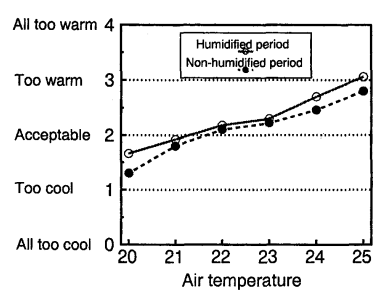
\includegraphics[scale=0.8]{img/tempHumidGraph.png}
    \caption{Luchttemperatuur in een wel en niet bevochtigde ruimte volgens de mening van werknemers\cite{palonen1993effects}}
\end{figure}


\subsection{Geluidsniveau}
Het geluidsniveau wordt gemeten in decibel met de A-weging (dBA)\cite{aWeighting}. De A-weging wordt gebruikt omdat het menselijk gehoor niet over alle frequenties geluid met dezelfde intensiteit ervaart. Om 68\% van de mensen tevreden te houden met het geluidsniveau in een kantooromgeving moet het niveau niet hoger zijn dan wat er beschreven is in \autoref{tab:soundLevels}\cite{geluid-levels}. In \autoref{tab:soundLevels} is het gemiddelde niveau een gemiddelde van een metingen over 10 seconden. Elke gemeten waarde die 5 dBA boven het gemiddelde niveau piekt wordt opgeteld bij de piek index van het gemiddelde niveau. Deze metingen zijn meerdere keren per uur gedaan in de loop van 3 dagen in het onderzoek\cite{geluid-levels}. 

\begin{table}[ht]
    \centering
    \begin{tabular}{ c | c }
        Gemiddelde niveau (dBA) & Piek index\\
        \hline
        50 & 44 \\
        55 & 26 \\
        60 & 14 \\
        65 & 6  \\
        70 & 1 
    \end{tabular}
    \caption{Gemiddelde waardes en piek indices}
    \label{tab:soundLevels}
\end{table}


\subsection{Lichtkwaliteit}

Lichtkwaliteit bestaat volgens de Europese regelgevingsnormen uit verschillende aspecten\cite{lightingIndorWorkspaces}. Een van deze aspecten is lichtintensiteit in lux, deze waarde verschilt per ruimte in een kantooromgeving. In \autoref{tab:lightLevelsOffices} zijn de waardes te zien waar een ruimte aan moet voldoen \cite{lightingIndorWorkspaces}.

\begin{table}[ht]
    \centering
    \begin{tabular}{ l | c }
        Type van interieur, taak of activiteit & Lux waarde\\
        \hline
        Archiveren, kopiëren, enz. & 300 \\
        Schrijven, typen, lezen, data verwerken & 500 \\
        Technische tekening & 750 \\
        CAD-Werkplekken & 500  \\
        Conferentie- en vergaderzalen (Verlichting moet regelbaar zijn) & 500  \\
        Receptiebalie & 300 \\
        Archieven & 200 

    \end{tabular}
    \caption{Licht vereisten in een kantooromgeving\cite{lightingIndorWorkspaces}}
    \label{tab:lightLevelsOffices}
\end{table}

\subsection{Metaconclusie}

Voor de metaconclusies zijn er twee factoren gekozen, luchtkwaliteit en kamertemperatuur. Als de VOC waarde boven de 3.0 \(mg/m^3\)  \cite{voc-luchtkwaliteit} en/of de luchtvochtigheid boven 60\%\cite{palonen1993effects} komt terwijl de kamertemperatuur boven de 22.9 $^{\circ}$C\cite{palonen1993effects} is, dan wordt er een advies gegeven om het raam open te zetten. 

% Noem 1 of 2 als voorbeeld
% Maak duidelijk dat dit een Proof of concept.


% Het uiteindelijk ontwerp bestaat uit 2 delen. De sensor data en het netwerk om de sensor data door te sturen. Beide moeten onderzocht worden, want beide zijn belangrijk.
% Uit beide onderdelen zullen ook specificaties komen om hiermee door te gaan naat het ontwerp gedeelte.

% \subsection{Sensor data}
% Te lezen in Hoofdstuk \ref{sec:assignment} is dat er dus een probleem is met comfortabelheid in een ruimte. In de probleemstelling is al kort verteld welke grootheden hier invloed op hebben. Dit waren temperatuur, luchtkwaliteit, licht en geluid. Dit zijn ze daarentegen niet allemaal. In het is te zien dat hij is gaan kijken naar de productiviteit van werknemers binnen een bedrijf. Uit dit onderzoek is gebleken dat werknemers minder productief zijn als de temperatuurboven de 20 graden is. Bij elke graad staat dat de productiviteit daalt met 4\%. Ook is een werknemer gemiddeld 6\% productiver in een rustigeen stille ruimte dan een werknemer die in een ruimte zit waar veel geluid te horen is en waar veel velle kleuren te zien zijn. \\

% Deze grootheden opzichzelf zijn al niet zo fijn, maar combintaties hiervan zullen nog erger zijn. Als er bijvoorbeeld wordt gekeken naar
% temperatuur opzichzelf dan kan dat niet comfortabel zijn bij bijvoorbeeld 24 graden, maar iemand zou hier nog gewoon in kunnen werken. 
% Als de factor luchtvochtigheid bij komt kijken dan is het ineens een ander verhaal. Dan kan het voor de gebruiker erg benauwd aan kunnen
% voelen en is de ruimte hierdoor dus niet meer fijn en productief om in te werken. Bijvoorbeeld de combinatie licht en geluid kan er na 
% een tijdje voor zorgen dat iemand hoofdpijn kan krijgen. Luchtkwaliteit en luchtvochtigheid kan ook voor een benauwd gevoel zorgen. \\

% Dit zijn goeie grootheden om te gebruiken in het netwerk. Maar de gebruiker moet ook feedback terug krijgen over de waardes die worden
% gemeten en eventueel horen of zien dat het niet meer productief is om in de ruimte te blijven. Hiervoor is een basisstation nodig. 
% Op dit station zou alle data binnen moeten komen. De gebruiker kan hier dus sowieso de waardes op uitlezen. Alleen is het logisch dat
% een gebruiker het verschil tussen 13 of 18 microgram per cubic meter. Wat in dit geval volgens de KNMI \cite{Gezonde} een verschil is tussen
% "de luchtkwaliteit is prima" en "de luchtkwaliteit is niet meer gezond". Hierdoor moet er voor elke parameter een kleine waarschuwing krijgen
% wanneer een bepaalde waarde is bereikt. Als er bijvoorbeeld wordt gekeken naar een telefoon en hoe deze meldingen laat zien dan zijn er 
% verschillende methodes om dat te doen. Dit wordt gedaan door een geluidje om de aandacht te trekken of door het scherm op te lichten. Soms
% is alleen dat niet genoeg en gaat de telefoon trillen en er is ook een mogelijkheid om een knipperende scherm melding te krijgen.

% \subsection{Netwerk}

% Bij het ontwerpen van een netwerk zijn er verschillende dingen om rekening mee te houden. De volgende onderdelen zijn standaarden voor netwerken: 

% \begin{itemize}
%     \item Bandbreedte: Dit verwijst naar de hoeveelheid gegevens die over het netwerk kunnen worden verzonden in een bepaalde tijdseenheid, gemeten in bits per seconde (bps), kilobits per seconde (Kbps), megabits per seconde (Mbps) of gigabits per seconde (Gbps). \cite{Bandbreedte}
%     \item Latentie: Dit is de vertragingstijd tussen het verzenden van gegevens vanaf de bron naar de bestemming. Lage latentie is cruciaal voor real-time toepassingen zoals videoconferenties of online gaming. \cite{Bandbreedte}
%     \item Beveiliging: Een manier om de data veilig te houden, zoals firewalls, encryptie en authenticatieprotocollen.
%     \item Schaalbaarheid: Het vermogen van het netwerk om te kunnen groeien en omgaan met een toename van gebruikers, apparaten en gegevensverkeer.
%     \item Betrouwbaarheid: Het vermogen van het netwerk om consistentie en beschikbaarheid te bieden, zelfs bij storingen of hoge belasting.
%     \item Datalink-snelheid: De maximale snelheid waarmee gegevens kunnen worden overgedragen tussen apparaten in het netwerk, vaak uitgedrukt in Mbps of Gbps.\cite{Data}
%     \item IP-adressering: De methode waarmee apparaten in het netwerk worden geïdentificeerd, meestal via IPv4- of IPv6-adressen.\cite{IP}
%     \item Mobiliteit: Voor draadloze netwerken, het vermogen van apparaten om naadloos tussen verschillende toegangspunten te schakelen zonder de verbinding te verliezen.
%     \item QoS (Quality of Service): Het vermogen van het netwerk om prioriteit te geven aan bepaalde soorten gegevensverkeer, zodat essentiële toepassingen soepel kunnen blijven werken, zelfs tijdens periodes van zware belasting.
%     \item Management en Monitoring: Het vermogen om het netwerk te monitoren en te beheren, inclusief tools en software die worden gebruikt voor netwerkbeheer.

% \end{itemize}
